\section{Quantum errors: Noise and Decoherence}
The Schrödinger equation
$$
i \hbar \frac{d|\psi\rangle}{d t}=H|\psi\rangle
$$
describes the evolution of quantum systems in isolation, where $|\psi\rangle$ is the state vector. These closed systems have a well-defined Hamiltonian operator $H$, which gives complete information about how these systems evolve. The resulting evolution is unitary: the evolution of the state is given by a linear map $|\psi(0)\rangle \rightarrow|\psi(t)\rangle=U|\psi(0)\rangle$ where $U^{\dagger} U=$ $U U^{\dagger}=I$. Note that these Hamiltonians may "come from outside" the system; for instance, we can turn external fields on and off, shine lasers, etc. What makes a quantum system closed is that it doesn't act back on the external world. The external fields, lasers, etc., can all be treated as classical potentials.

The unfortunate reality is that this idealization is fiction. All real quantum systems interact with the outside world, at least weakly; and the existence of interactions, which allow us to manipulate a system, also allows the system to interact with the external environment. This uncontrolled environmental interaction is called decoherence.

One can model the dynamics of a register of qubits with its surroundings. We imagine the system immersed into its environment (often called bath) and the whole (quantum register plus environment) as a closed system described in a general way by the following Hamiltonian:
$$
H=H_{S} \otimes I_{B}+I_{S} \otimes H_{B}+H_{\mathcal{I}}
$$
where $H_{S}\left(H_{B}\right)$ (the system (bath) Hamiltonian) acts on the system (bath) Hilbert space $\mathcal{H}_{S}$ $\left(\mathcal{H}_{B}\right), I_{S}\left(I_{B}\right)$ is the identity operator on the system (bath) Hilbert space, and $H_{I}$, which acts on both the system and bath Hilbert spaces $\mathcal{H}_{S} \otimes \mathcal{H}_{B}$, is the interaction Hamiltonian containing all the nontrivial couplings between system and bath. In general, $H_{\mathcal{I}}$ can be written as a sum of operators which act separately on the system $\left(S_{\alpha}\right.$) and on the bath $\left(B_{\alpha}\right.$) \cite{kempe2006approaches}:
$$
H_{\mathcal{I}}=\sum_{\alpha} S_{\alpha} \otimes B_{\alpha}
$$
In the absence of an interaction Hamiltonian $\left(H_{\mathcal{I}}=0\right)$, the evolution of the system and the bath are separately unitary: $\mathbf{U}(t)=\exp (-i \frac{H}{\hbar} t)=\exp \left(-i \frac{H_{S}}{\hbar} t\right) \otimes \exp \left(-i \frac{H_{B}}{\hbar} t\right)$ . Information that has been encoded (mapped) into states of the system Hilbert space remains encoded in the system Hilbert space if $H_{\mathcal{I}}=0$.
 However, in the case when the interaction Hamiltonian contains nontrivial couplings between the system and the environment ($H_{\mathcal{I}}\neq 0$), decoherence can happen. %information that has been encoded over the system Hilbert space does not remain encoded over solely the system Hilbert space but spreads out instead into the combined system and bath Hilbert space as the time evolution proceeds.

Two things can cause decoherence. First, random influences from the outside can perturb the system's evolution, as if some random Hamiltonian was turned on, in addition to the usual Hamiltonian. Second, the interaction between the system and environment can cause information about the system to leak into the environment. This information leakage leaves the system correlated with the environment. In fact, a certain quantity of information that was previously carried by the system, then is spread out also in the environment. The No-hiding theorem shows how this property works. The effect on the system is as if unwanted measurements have been performed (without, in general, our knowing the measurement results).
In fact, these two processes generally both occur, and their practical effects often look similar. Indeed, in quantum mechanics, there is no sharp distinction between them. If decoherence persists long enough, it is possible for all information about the original state of the system to be lost. In the shorter term, decoherence can destroy quantum effects such as interference and entanglement (on which quantum information processing depends).

In general, we can study the evolution of an isolated quantum systems subjected to decoherence and other sources of noise using quantum states, but as already said in the previous section, the state vector approach does not immediately allow for a formalisation of ignorance or missing knowledge. A more general description can be done using the density matrix formalism.

Maps that represent the evolution of the density operator must preserve certain properties: they are completely positive, trace-preserving and map density matrix into density matrix.
Maps that satisfy these properties are called CPTP maps and can be written as:
$$
\rho' = \mathcal{E}(\rho) \rightarrow \sum_{\mu} K_{\mu} \rho K_{\mu}^{\dagger} \quad \text { with } \sum_{\mu} K_{\mu}^{\dagger} K_{\mu}=I
$$
where the $K_{\mu}$ are $N \times N$ matrices ($N$ being the dimension of the Hilbert space) and are called Kraus operators. 
In general, the Kraus decomposition of a CPTP map is not unique, but one can approximately think of the map as the state $|\psi\rangle$ being multiplied by one of the operators $K_{\mu}$ chosen at random with probability $p_{\mu}=\bra{\psi} K_{\mu}^{\dagger} K_{\mu}\ket{\psi} .$ Since one does not know which operator has acted on the state, one uses a mixture of all of them.

Similarly, if an unknown influence is applied to the quantum system from the outside, we can model that as a set of unitaries $\left\{A_{\mu}\right\}$ that occur with respective probabilities $\left\{p_{\mu}\right\}$. Here, again, one would describe the state of the system as a mixture of all possible evolved states:
$$
\rho \rightarrow \rho^{\prime}=\sum_{\mu} p_{\mu} A_{\mu} \rho A_{\mu}^{\dagger}, \quad \sum_{\mu} p_{\mu}=1
$$
In this case, again we have a CPTP map, and we can define the Kraus operators to be $K_{\mu} \equiv \sqrt{p_{\mu}} A_{\mu} .$ 
CPTP maps give a unified description of all possible sources of Markovian noise\footnote{ Markovian dynamics means a limit or approximation in which the recent details do not matter, that is, the environment is "memoryless" and does not contain information about the history of the system. This is advantageous because it allows us to write an equation for $\rho(t)$ that depends only on $\rho(t)$, and not on, say, $\rho\left(t-t^{\prime}\right)$. This is called "time local" equation and is much easier to handle.}, and in quantum information science one does not usually make a sharp distinction between different noise sources. 




\section{Fidelity}
In communication problems, we would like to know how much information is preserved by some processes. We would like to compare the initial message and the final message after the effect of noise. 
A quantity that can represent the similarity between two states is fidelity. 
Hence, it is possible to use fidelity as an appropriate measure of the quality of a recovered code.

The fidelity can be written as the overlap between the final state $\rho_f$ of a system $\rho$ and the original state $\ket{\psi}$.
If the combined operator consisting of an interaction with the environment ($E_a$) followed by a recovery operation ($\mathcal{R}_a$) is given by $\mathcal{A}=\left\{A_{a}=\mathcal{R}_aE_a, \ldots\right\}$\footnote{The subscription $a$ indicates a generic error $E_a$ as kraus operator, followed by its recovery procedure $\mathcal{R}_a$. If we want to study the case where there is no recovery for that error we put $\mathcal{R}$ equal to the identity operator, getting only the action of error in the fidelity}, then:
$$
\mathcal{F}\left(\rho_f,\ket{\psi_i}\right)=\bra{\psi_i}\rho_{f}\ket{\psi_i}=\sum_{a}\bra{\psi_i}A_{a}\ket{\psi_i}\bra{\psi_i}A_{a}^{\dagger}\ket{\psi_i} .
$$
It gives the probability that the final state would pass a test checking whether it agrees with the initial state \cite{Knill_2000}. As we are thinking of encoding arbitrary states, we do not know in advance the state that will be used. We, therefore, use the minimum fidelity (that is the worst-case fidelity)
\begin{equation}
\mathcal{F}_{\min }=\min _{|\psi\rangle}\left\langle\psi\left|\rho_{f}\right| \psi\right\rangle .
\end{equation}
The best quantum code maximizes $\mathcal{F}_{\min }$. 


A quantum communication channel can be used to transmit the state $\ket{\psi}$ from one location to another. No channel is ever perfect, so its action is described by a quantum operation $\mathcal{E}$ on $\rho=\ket{\psi}\bra{\psi}$.

Let's take an example of a noisy channel: the depolarising channel denoted as $\mathcal{D}$. This channel leaves the qubit untouched with probability $1-p$ and with probability $\frac{p}{3}$ one of the 3 errors $\{X,Y,Z\}$ can act on the qubit: 
\begin{equation}
    \rho'=\mathcal{D}(\rho) = (1-p)\rho + \frac{p}{3}\left(X\rho X +Y \rho Y+Z \rho Z\right)
\end{equation}
We can rewrite the expression as: 
$$
\begin{aligned}
\rho^{\prime} &=\frac{p}{3}(X \rho X+Y \rho Y+Z \rho Z)+(1-p) \rho \\
&=\frac{p}{3}(\rho+X \rho X+Y \rho Y+Z \rho Z)+\left(1-\frac{4 p}{3}\right) \rho. \\
\end{aligned}
$$
We can further simplify the expression more, using the following relation\footnote{It is straightforward to calculate that $\mathcal{E}(I)=I$ and $\mathcal{E}(X)=\mathcal{E}(Y)=\mathcal{E}(Z)=0$. However, $I, X, Y, Z$ form a basis of $2\times2$ matrices, so any $\rho$ can be written as $\rho=a I+b X+c Y+d Z$ and then $\mathcal{E}(\rho)=a I$. If $\rho$ is a density matrix then $a=\frac{1}{2}$ and $\mathcal{E}(\rho)=I / 2$. This means that $\mathcal{E}$ maps a pure state into a mixed state, for example $\mathcal{E}(\ket{0}\bra{0}) =\frac{1}{2}(\ket{0}\bra{0} + \ket{1}\bra{1})$}: 
$$
\frac{1}{4}(\rho+X \rho X+Y \rho Y+Z \rho Z)=\frac{I}{2}.
$$
Then, we can use this result and put it in the previous equations: 
$$
\begin{aligned}
&\rho'=\frac{4 p}{3} \frac{I}{2}+\left(1-\frac{4 p}{3}\right) \rho \\
&=\lambda \frac{I}{2}+(1-\lambda) \rho
\end{aligned}.
$$

Here, $\lambda=\frac{4 p}{3} \in\left[0, \frac{4}{3}\right]$ is the depolarization parameter. Equivalently, the depolarizing channel can also be described as replacing the state with a completely mixed state with a chance of $\lambda = \frac{4p}{3}$. The effect of this error channel on the Bloch sphere (figure \ref{fig:depchannel}) can therefore be thought as an isotopical shrinking of the sphere. 

\begin{figure}[h!]
    \centering
    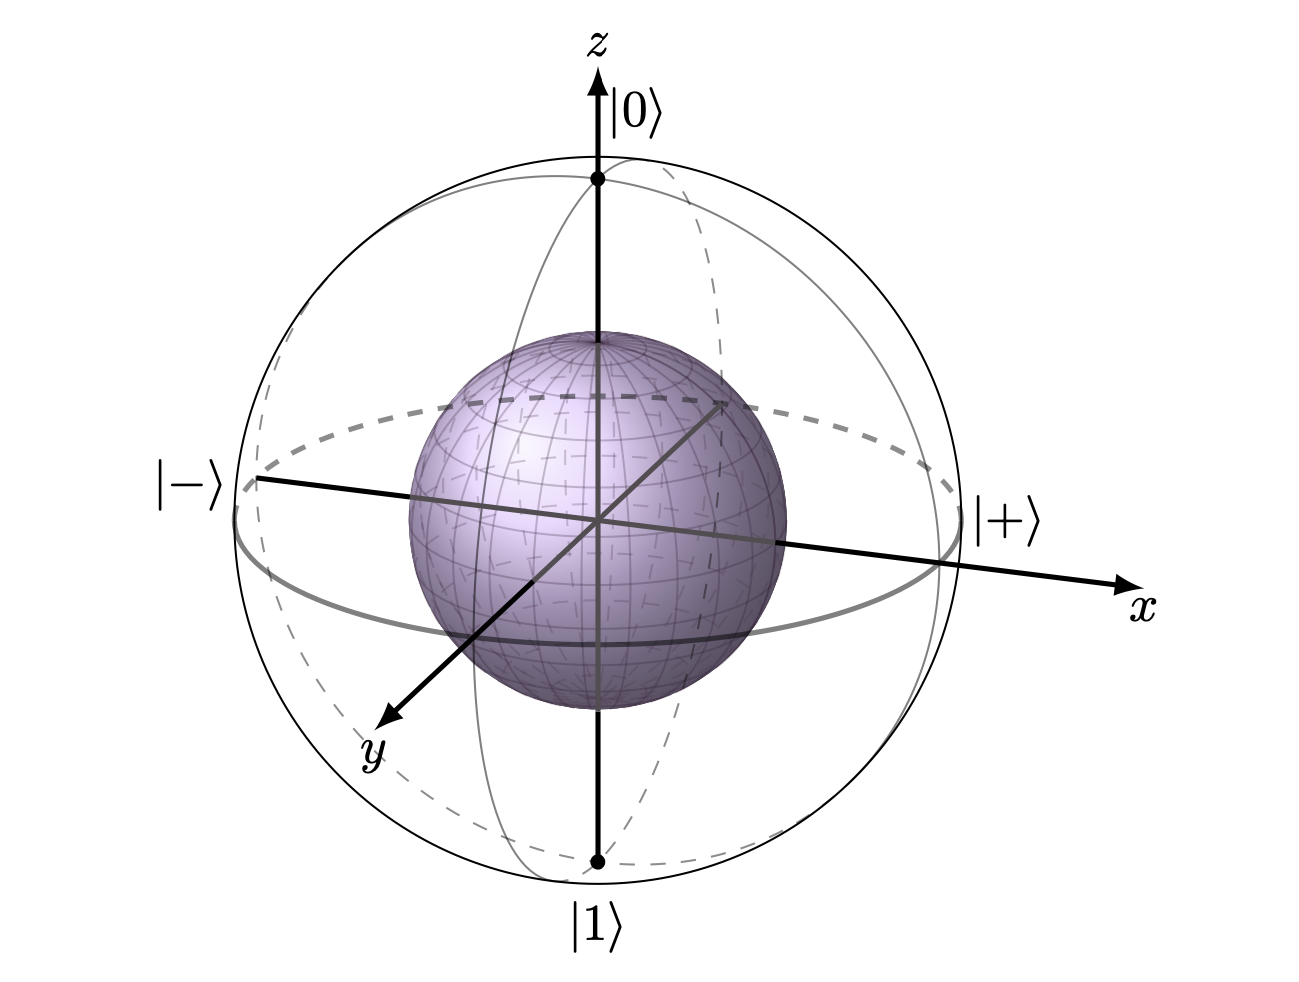
\includegraphics[scale=0.5]{Mainmatter/images/Depolarizing_channel.png}
    \caption{
The depolarizing channel has the same probability for each type of error to occur. Consequently, the effect on the Bloch sphere is isotropic: the sphere is rescaled by a factor of $(1-p)$. Since the depolarizing channel also has the interpretation of replacing a qubit with a completely mixed state, its outcome will always be an ensemble that is closer to the Bloch sphere’s center than the original density operator.}
    \label{fig:depchannel}
\end{figure}
From this we can calculate the fidelity between the initial and final mixed state: 
\begin{align*}
    \mathcal{F}(\ket{\psi},\rho') &= \text{min}_{\ket{\psi}}  \bra{\psi}\rho'\ket{\psi} \\
    &= \bra{\psi}(\lambda \frac{I}{2}+(1-\lambda) \ket{\psi}\bra{\psi})\ket{\psi} \\
    &= \frac{\lambda}{2} + (1-\lambda) = 1-\frac{2}{3}p .
\end{align*}
This result agrees with our intuition: the higher the probability $p$ of depolarizing, the lower the fidelity is. For a very small $p$ the fidelity is closer to one, and the state $\mathcal{E}(\rho)$ is practically indistinguishable from the initial state. More examples can be done using different channels can be studied in the same way.


% So far, we have looked only when the state sent into the channel is not entangled, but in quantum error correcting code in order to protect a qubit we have to entangle it. 
% The states to be protected involve a subset of entangled qubits. This means that in discussions of fidelity and error, the whole state, not just the component being protected, must be considered.
% The worst case fidelity for such states is referred to as the entangled state fidelity to distinguish it from the pure state fidelity introduced earlier.
% If the pure state fidelity after recovery of the coded subsystem is one, then the entangled state fidelity is one also; it does not matter if the state is pure or if it is entangled with other systems. This observation is invalid if we have imperfect fidelity.
% %We can also characterize the channel by introducing a reference qubit $R$ and describing how a maximally-entangled state of the two qubits $RA$ evolves, when the channel acts only on $A$. There are four mutually orthogonal maximally entangled states, They also form a basis and are called Bell's states. 
% %If the initial state is $\left|\phi^{+}\right\rangle_{R A}$, then when the depolarizing channel acts on qubit $A$, the entangled state evolves as
% % $$
% % \left|\phi^{+}\right\rangle\left\langle\phi^{+}|\mapsto(1-p)| \phi^{+}\right\rangle\left\langle\phi^{+}\right|+\frac{p}{3}\left(\left|\psi^{+}\right\rangle\left\langle\psi^{+}|+| \psi^{-}\right\rangle\left\langle\psi^{-}|+| \phi^{-}\right\rangle\left\langle\phi^{-}\right|\right) .
% % $$
% Consider a quantum system of combined two quantum subsystems labeled
% as $A$ and $B$. The state of $A$ is assumed to be entangled in some way with the external world that we indicates with $B$. Suppose the joint system $AB$ initially is prepared in a general state $\rho_{i}=\ket{\psi_{AB}}\bra{\psi_{AB}}$. This is an entangled state, and we would like to know how well an entangled state is preserved after the action of noise.
% Assume that only the subsystem $A$ is affected by the noisy channel with
% some evolution described by a quantum operation $\mathcal{E} = \{E_a\}$, for example it can be a bit flip with probability $p_a$. While the subsystem $B$
% is dynamically isolated. In this case, the overall dynamics of the joint system $AB$ is described by the quantum operation $\mathcal{E} \otimes I$, where $I$ here is the identity operator acting on the subsystem $B$. Thus the final state of the joint system is given by the density operator $\rho_{\mathrm{f}}= \mathcal{E}\left(\rho_{\mathrm{i}}\right) \otimes I $.
% Such as for the isolated state, we can compute the fidelity for an entangled state $\mathcal{F}_e$ as well.
% \begin{equation}
% \mathcal{F}_{e}(\ket{\psi_{AB}},\rho_f)=\min _{\left|\psi_{AB}\right\rangle }\left\langle\psi_{AB}\left|\rho_f\right| \psi_{AB}\right\rangle
% \label{eq:entfidel}
% \end{equation}
% The $\mathcal{F}_e$, in fact, takes its value in the interval $[0, 1]$, where values close to 1 are supposed to imply that the entanglement is well preserved and values close to $0$ indicate that the entanglement is mostly destroyed.
% Using the operation sum representation the action of noise on the initial state is :
% \begin{equation*}
% \rho_f=(\mathcal{E}\otimes I)(\rho)=\sum_{a} E_a\ket{\psi_{AB}}\bra{\psi_{AB}} E_a^{\dagger}\end{equation*}
% Then, we can substitute this in eq(\ref{eq:entfidel}): 
% \begin{align*}
%     \mathcal{F}_e&=\text{min}_{\psi_{AB}} \sum_a  \bra{\psi_{AB}}E_a\ket{\psi_{AB}}\bra{\psi_{AB}} E_a^{\dagger}\ket{\psi_{AB}} \\&= \text{min}_{\psi_{AB}} \sum_a  |\bra{\psi_{AB}}E_a\ket{\psi_{AB}}|^2
% \end{align*}
% Then, we can write the entangled state in the Schmidt basis as $\left|\psi_{AB}\right\rangle=\sum_{i} \sqrt{p_{i}}\left|\psi_{i}^{A}\right\rangle\left|\psi_{i}^{B}\right\rangle$:
% \begin{align*}
%     \bra{\psi_{AB}}E_a\ket{\psi_{AB}} &= \sum_{ij} \sqrt{p_i p_j} \braket{\psi_i^B|\psi_j^B} \braket{\psi_i^A|E_a|\psi_j^A}\\ 
%     &= \sum_i p_i \braket{\psi_i^A|E_a|\psi_i^A}\\
%     &= Tr(\rho E_a)
% \end{align*}
% Hence: 
% \begin{equation}
%     \mathcal{F}_e = \sum_a \left(Tr(\rho E_a)\right)^2
% \end{equation}

% Thus, for example, consider the interaction consisting of scalar multiples of the Pauli spin matrices,
% $$
% \mathcal{E}=\left\{\frac{1}{\sqrt{3}} X, \frac{1}{\sqrt{3}} Y, \frac{1}{\sqrt{3}} Z\right\} .
% $$
% We show that for this example, $F(\mathcal{E})=\frac{1}{3}$ (Fidelity for a not entangled state) and
% $F_{e}(\mathcal{E}(\rho))=0 $  (entangled fidelity).

% Consider the general state $|u\rangle=$ $\alpha|0\rangle+e^{i \theta} \beta|1\rangle$ with $\alpha$ and $\beta$ real, and $\alpha^{2}+\beta^{2}=1$. The fidelity $\mathcal{F}(\mathcal{E}(\rho), \ket{u})$ is obtained by the following expression
% $$
% \begin{aligned}
% \mathcal{F}=\frac{1}{3}\left(\left|\left\langle u\left|X\right| u\right\rangle\right|^{2}\right.&\left.+\left|\left\langle u\left|Y\right| u\right\rangle\right|^{2}+\left|\left\langle u\left|Z\right| u\right\rangle\right|^{2}\right) \\
% &=\frac{1}{3}\left((2 \alpha \beta \cos (\theta))^{2}+(2 \alpha \beta \sin (\theta))^{2}+\left(\alpha^{2}-\beta^{2}\right)^{2}\right)
% \end{aligned}
% $$
% $$
% \begin{array}{l}
% =\frac{1}{3}\left(\left(\alpha^{2}+\beta^{2}\right)^{2}\right) \\
% =\frac{1}{3} .
% \end{array}
% $$
% Hence $F(\mathcal{E}(\rho),\ket{u})=\frac{1}{3}$. Then let us calculate the entangled fidelity considering as initial state the completely entangled state $|e\rangle=\frac{1}{\sqrt{2}}(|0\rangle|0\rangle+|1\rangle|1\rangle) .$
% Then the entangled fidelity $F_{e}(\mathcal{E}(\rho),\ket{e})$ is given by \ref{eq:entfidel}, where we apply $\mathcal{E}$ only to the system A: 
% $$
% \begin{aligned}
%  \sigma_{x} \otimes I|e\rangle &=\frac{1}{\sqrt{2}}(|0\rangle|1\rangle+|1\rangle|0\rangle) \\
% \sigma_{y} \otimes I|e\rangle &=\frac{i}{\sqrt{2}}(|0\rangle|1\rangle-|1\rangle|0\rangle) \\
% \sigma_{z} \otimes I|e\rangle &=\frac{i}{\sqrt{2}}(|0\rangle|0\rangle-|1\rangle|1\rangle)
% \end{aligned}
% $$
% These states are all orthogonal to $|e\rangle$, hence $F_{e}(\mathcal{E}(\rho))=0$.